\documentclass[aspectratio=169]{beamer}
%\usetheme{Marburg}
\usepackage[utf8]{inputenc}
\usepackage[russian]{babel}
\usepackage[OT1]{fontenc}
\usepackage{amsmath}
\usepackage{amsfonts}
\usepackage{amssymb}
\usepackage{graphicx}
\usepackage{mathtools}
\usepackage{xcolor}
\usepackage{empheq}
\usepackage[many]{tcolorbox}
\usepackage{multirow}

\usepackage{tikz}
\usetikzlibrary{shadings,shadows,shapes.arrows}

\newcommand*{\tikzarrow}[2]{%
  \tikz[
    baseline=(A.base),             % Set baseline to the baseline of node content
    font=\footnotesize\sffamily    % Set fontsize of the node content
  ]
  \node[
    single arrow,                  % Shape of the node
    single arrow head extend=5pt,  % Actual width of arrow head
    draw,                          % Draw the node shape
    inner sep=3pt,                 % Separation between node content and node shape
    top color=#1,               % Shading color on top of node
    bottom color=#1,               % Shading color on bottom of node
    % drop shadow                    % Draw a shadow
  ] (A) {#2};%
}

\newcommand{\tikzfancyarrow}[2][2cm]{\tikz[baseline=-0.5ex]\node [arrowstyle=#1] {#2};}

\author{Николай Анохин}

\title{Задача и алгоритмы кластеризации}
%\setbeamercovered{transparent} 
\setbeamertemplate{navigation symbols}{} 
%\logo{} 
%\institute{} 
\date{} 
%\subject{}

\tcbset{highlight math style={enhanced,colframe=red,colback=white,arc=4pt,boxrule=1pt}}

\setbeamertemplate{caption}{\raggedright\insertcaption\par}

\newcommand*\rot{\rotatebox{90}}

\begin{document}

\begin{frame}
\titlepage
\end{frame}

\begin{frame}{Обучение без учителя}

В задачах {\bf без учителя} значение целевой функции для объектов из обучающей выборки неизвестно. Решение таких задач подразумевает исследование ``скрытой структуры'' данных.

\vspace{2em}
Задача {\bf кластеризации} -- задача без учителя, подразумевающая разбиение множества объектов на непересекающиеся подмножества (кластеры).

\end{frame}

\begin{frame}{Мотивация}

\begin{itemize}
\item
\only<1>{Кластеризация позволяет больше узнать о данных (knowledge discovery!)}
\only<2>{Работать с кластерами удобнее, чем c отдельными объектами}
\only<3>{Кластеризация позволяет конструировать новые признаки}
\end{itemize}

\only<1>{
\begin{figure}
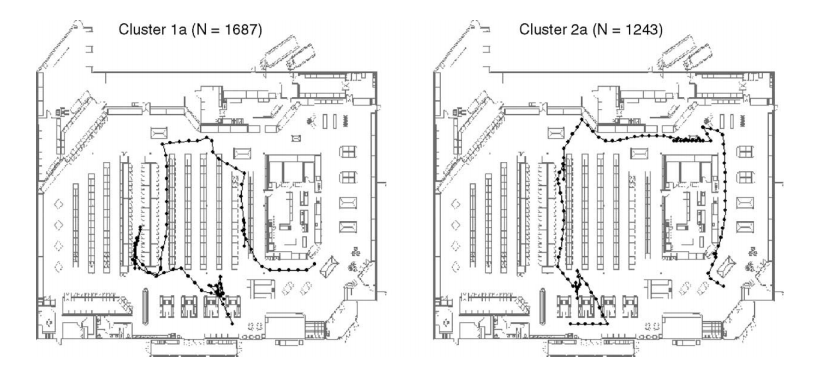
\includegraphics[width=0.8\textwidth]{images/paths.png}
\caption{Типичные траектории покупателей супермаркета\footnote{\href{https://statistics.wharton.upenn.edu/files/?whdmsaction=public:main.file&fileID=346}{An exploratory look at supermarket shopping paths // J.S. Larson et. al.}}}
\end{figure}
}
\only<2>{
\begin{figure}
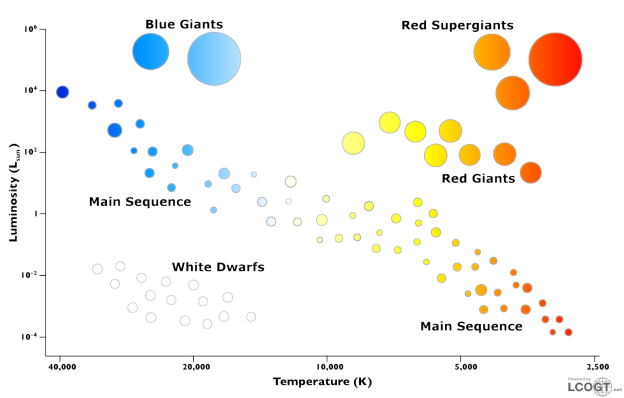
\includegraphics[height=0.55\textheight]{images/hrdiagram.png}
\caption{Диаграмма Герцшпрунга — Рассела\footnote{\url{https://lcogt.net/spacebook/h-r-diagram/}}}
\end{figure}
}
\only<3>{
\begin{quote}
\texttt{d1: Банк финансирует строительство футбольного стадиона} \\
\texttt{d2: Автомобили подорожали из-за финансового кризиса } \\
\end{quote}
\vspace*{\fill}
\begin{tabular}{r | c c c c c c c c c}
 & \rot{\it банк} & \rot{\it финансы} & \rot{\it строительство} & \rot{\it футбол} & \rot{\it стадион} & \rot{\it автомобиль} & \rot{\it подорожание} & \rot{\it кризис} & \ldots \\
\hline
\texttt{d1} & 1 & 1 & 1 & 1 & 1 & 0 & 0 & 0 & \ldots \\
\texttt{d2} & 0 & 1 & 0 & 0 & 0 & 1 & 1 & 1 & \ldots \\
& \multicolumn{9}{c}{\ldots}
\end{tabular} \quad \tikzarrow{pink}{clustering} \quad
\begin{tabular}{r | c c c c}
 & \rot{\it экономика} & \rot{\it спорт} & \rot{\it производство} & \ldots \\
\hline
\texttt{d1} & 2 & 2 & 1 & \ldots \\
\texttt{d2} & 3 & 0 & 1 & \ldots \\
 & \multicolumn{4}{c}{\ldots}
\end{tabular}
}

\end{frame}

\begin{frame}{Задача кластеризации}

\vspace{1em}
{\bf Дано.} Признаковые описания $N$ объектов $\mathbf{x} = (x_1, \ldots, x_m) \in \mathcal{X}$, образующие тренировочный набор данных $X$

\vspace{1em}
{\bf Найти.} Модель из семейства параметрических функций 
\[
H = \{h(\mathbf{x, \mathbf{\theta}}): \mathcal{X} \times \Theta \rightarrow \mathcal{Y} \mid \mathcal{Y} = \{1, \ldots, K\}\},
\]
ставящую в соответствие произвольному $\mathbf{x} \in \mathcal{X}$ один из $K$ кластеров так, чтобы объекты внутри одного кластера были похожи, а объекты из разных кластеров различались

\end{frame}

\begin{frame}

\begin{center}
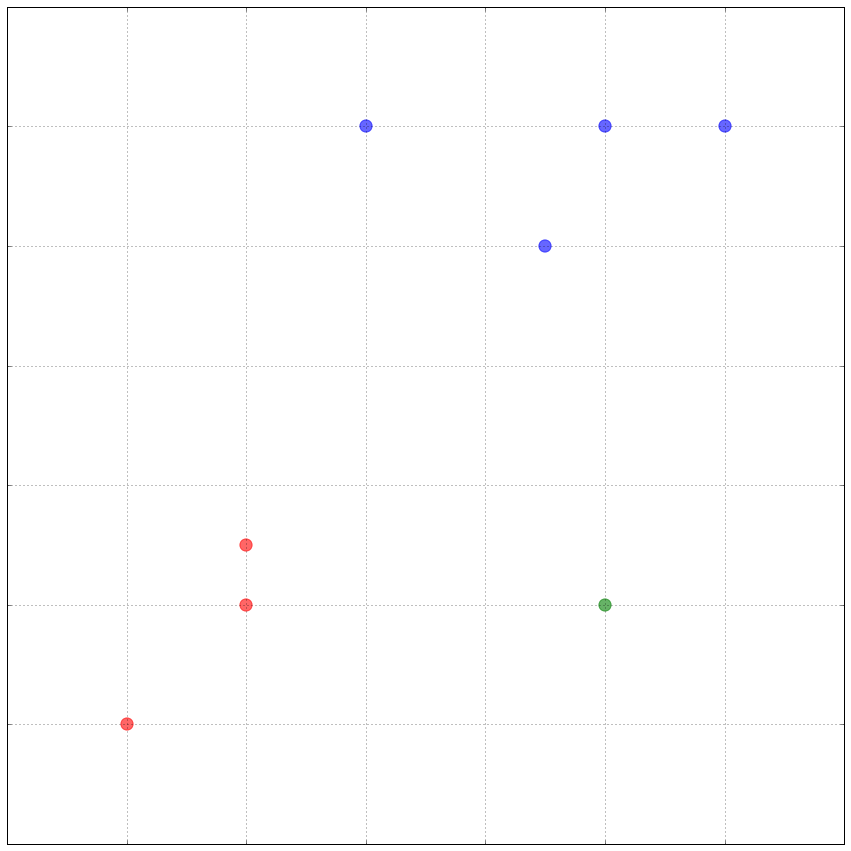
\includegraphics[height=0.9\textheight]{images/toy.png}
\end{center}

\end{frame}

\begin{frame}{Иерархическая кластеризация}

{\bf Идея агломеративного алгоритма}
\begin{enumerate}
\item при инициализации считаем, что каждый объект --- отдельный кластер
\item на каждом шаге совмещаем два наиболее близких кластера
\item останавливаемся, когда получаем требуемое количество кластеров или остается единставенный кластер, содержащий все объекты
\end{enumerate}

\end{frame}

\end{document}